% Chapter 1

\chapter{Introducción} % Main chapter title

\label{Chapter1} % For referencing the chapter elsewhere, use \ref{Chapter1} 
\label{IntroGeneral}

%----------------------------------------------------------------------------------------

% Define some commands to keep the formatting separated from the content 
\newcommand{\keyword}[1]{\textbf{#1}}
\newcommand{\tabhead}[1]{\textbf{#1}}
\newcommand{\code}[1]{\texttt{#1}}
\newcommand{\file}[1]{\texttt{\bfseries#1}}
\newcommand{\option}[1]{\texttt{\itshape#1}}
\newcommand{\grados}{$^{\circ}$}

%----------------------------------------------------------------------------------------

%\section{Introducción}

%----------------------------------------------------------------------------------------
% Temas posibles a desarrollar:
%independencia de los bloques IP
% objetivo de introducir los automatismos
%	Blanco
%	Hit
%	Plot
%	Presencia
%	Pista o track

\section{Conceptos generales de radares}

\subsection{Radar}

El radar (acrónimo del inglés Radio Detection and Ranging), de acuerdo a la definición dada por ENACOM (Ente Nacional de Comunicaciones), es un sistema que permite determinar la localización y/o la velocidad de un objeto a través del uso de radiaciones electromagnéticas \citep{Enacom}. Estas ondas una vez emitidas en cierta dirección, cuando impactan en algún objeto, se reflejan en distintas direcciones. Una onda reflejada regresa al radar y contiene una pequeña parte de la energía emitida originalmente. De esta manera, conociendo la velocidad de propagación de la onda y midiendo el tiempo de retardo, se puede conocer datos del mismo, por ejemplo la posición relativa del objetivo y su velocidad.

En general se utiliza el sistema de coordenadas polares: proporciona el alcance y la orientación de los objetivos encontrados con respecto a la posición de la antena. Cabe mencionar que el rango es la distancia inclinada \citep{radar_tutorial_slant_range} desde la antena y no la distancia horizontal, como se ilustra en la figura \ref{Rango_figura}.
 
\begin{figure}
\centering
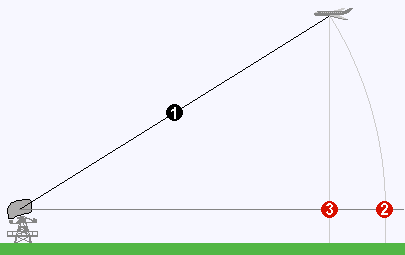
\includegraphics[scale=0.65]{./Figures/Slant_range.png}
\caption{Rango, altura y distancia a nivel de tierra. Imagen tomada de WolfgangW \citep{WolfgangW}. El rango inclinado (1) es la hipotenusa del triángulo representado por la altitud de la aeronave y la distancia entre la antena del radar y la trayectoria en tierra de la aeronave (punto (3) en la tierra directamente debajo de la aeronave). En ausencia de información de altitud, la ubicación de la aeronave se trazaría más lejos (2) de la antena que su trayectoria real en tierra.} 
\label{Rango_figura}
\end{figure}


El patrón de radiación de la antena se ilustra en la figura \ref{patrón_de_radiación} un haz estrecho cuando se ve desde arriba y, con cierta aproximación, puede considerarse como un trapecio si se ve de lado.


\begin{figure}
\centering
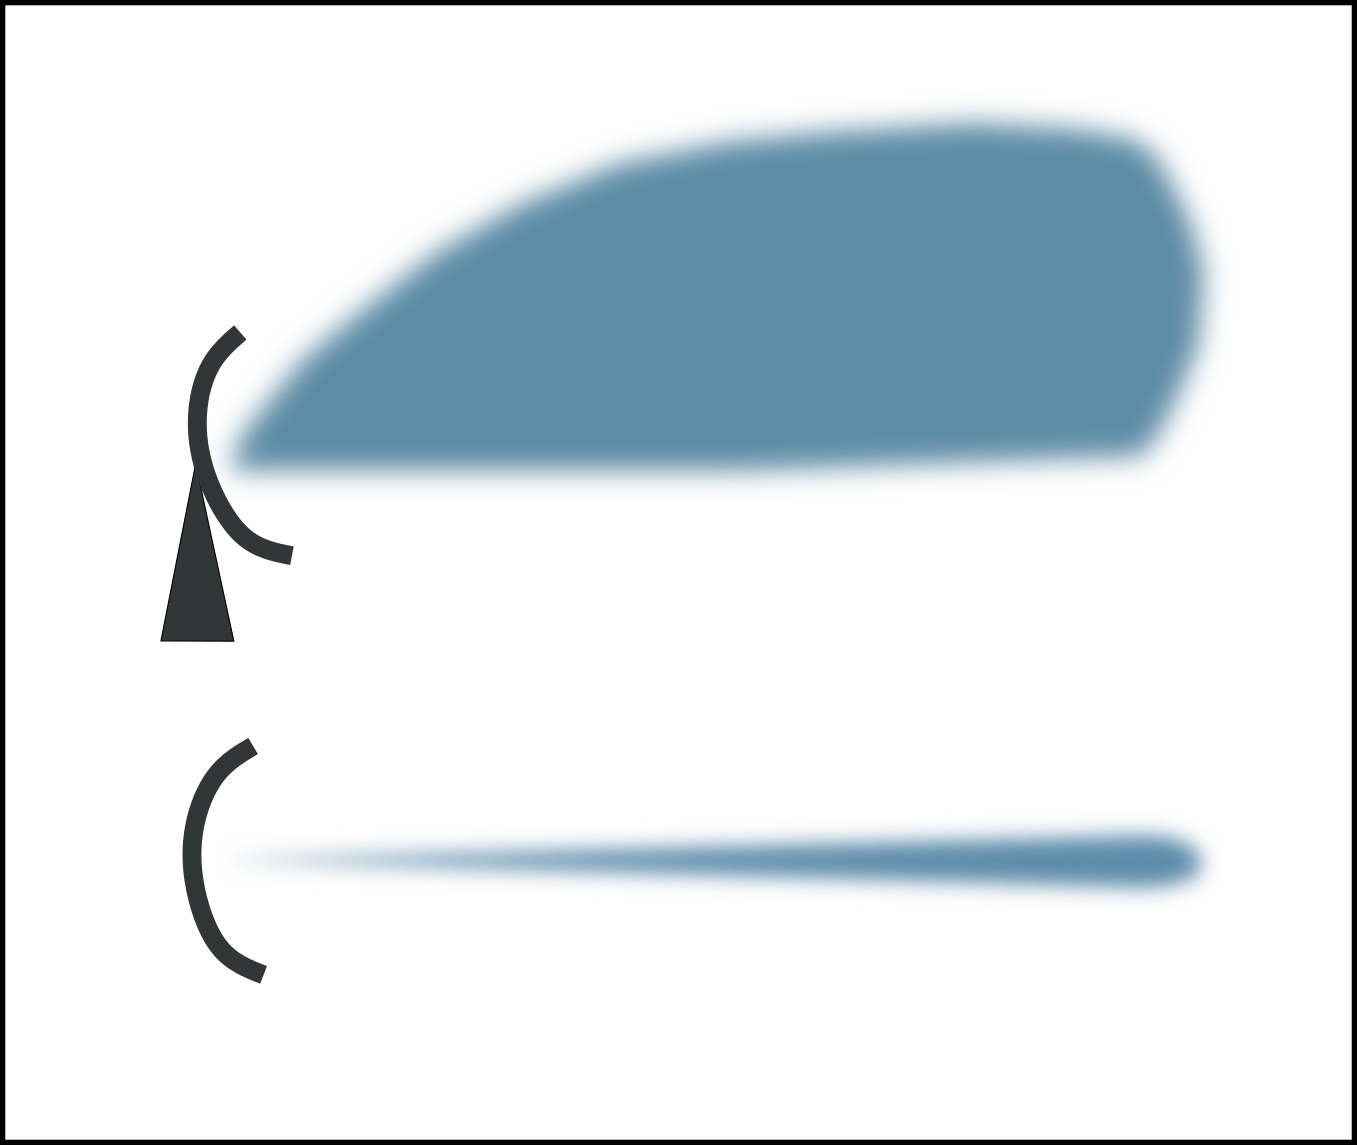
\includegraphics[scale=0.2]{./Figures/PSR_vistas.png}
\caption{Patrón de radiación de la antena.}
\label{patrón_de_radiación}
\end{figure}


Los radares que identifican objetos mediante la detección de reflexiones que estos producen de señales de radiofrecuencia se denominan radares primarios \citep{PSR}. Estos utilizan una antena que gira continuamente montada en una torre para transmitir ondas electromagnéticas que se reflejan, o se dispersan, desde la superficie de la aeronave hasta cierta cantidad de millas náuticas desde el radar. El sistema de radar mide el tiempo necesario para que el radar repita el eco y la dirección de la señal. A partir de esto, el sistema puede medir la distancia de la aeronave a la antena del radar y el azimut, o dirección, de la aeronave en relación con la antena.

Existen otro tipo de radares de vigilancia, denominados secundarios, que utilizan una segunda antena de baliza de radar unida a la parte superior de la antena del radar principal para transmitir y recibir datos del área de la aeronave para la altitud barométrica, el código de identificación y las condiciones de emergencia. Se emiten pulsos codificados, para realizar interrogaciones mediante trenes de pulsos. Las aeronaves militares, comerciales y algunas de aviación general tienen transpondedores que responden automáticamente a una señal del radar secundario informando un código de identificación y altitud. Los centros de control de tráfico aéreo utilizan estos datos del sistema para verificar la ubicación de la aeronave dentro de un radio determinado del sitio del radar. El radar secundario también proporciona una identificación rápida de aeronaves en peligro.

Se menciona a continuación algunas ventajas y desventajas de los radares primarios:
\begin{itemize}
\item
Ventajas
	\begin{itemize}
	\item
El radar primario es el único sensor de vigilancia utilizado en la aviación civil que no requiere ningún equipo a bordo para localizar la aeronave. A diferencia de radar secundario, puede descubrir una aeronave que experimente una falla de transpondedor o un intruso.
	\item
Se utiliza para captar objetivos de larga distancia. Puede detectar aviones desde una distancia de cientos de kilómetros.
	\item
Mantiene 360 grados de vigilancia desde la superficie hasta grandes altitudes. Determina la orientación de los objetivos en un área más grande.
	\end{itemize}

\item
Desventajas
	\begin{itemize}
	\item
	Cono de silencio. Debido al patrón de radiación, hay una parte del espacio aéreo sobre la antena que no se puede inspeccionar. Este efecto se mitiga colocando una serie de radares de tal manera que el cono de silencio de cada radar quede cubierto por otro radar.
	\item
	Los objetivos con el mismo rango de inclinación (en diferentes niveles) son difíciles de distinguir (las señales recibidas se superpondrán). Esto se mitiga combinando el radar primario con un radar secundario que puede reconocer las diferentes aeronaves por sus códigos de transpondedor.
	\item
	Límite de rango mínimo. El PSR opera en una frecuencia, lo que significa que no puede emitir y recibir señal al mismo tiempo. Si el objetivo está demasiado cerca de la antena del radar, la señal reflejada puede recibirse antes del final de la transmisión. Si eso sucede, el objetivo no será detectado. Tenga en cuenta que acortar el pulso también reducirá la cantidad de energía emitida, lo que limitará el alcance máximo del radar. Esto se mitiga ajustando la longitud del pulso y la velocidad de rotación de la antena.
	\end{itemize}
\end{itemize}


\subsection{Tipos de radares}
La tecnología de radar ha experimentado muchos cambios desde su invención. Actualmente existe diversa variedad de sistemas de radar \citep{RadarHandbook} que se pueden clasificar en varias categorías según la finalidad de uso, cantidad de antenas, dependencia del blanco (radares primarios y secundarios mencionados anteriormente), forma de onda, ámbito de aplicación, etc. A continuación se destacan algunos de los sistemas de radar más comunes:

\begin{itemize}
\item Radar biestático:
Consta de un transmisor y un receptor que están separados por una distancia que es igual a la distancia del objetivo esperado. Un radar en el que el transmisor y el receptor están ubicados en el mismo lugar se conoce como radar monoestático. La mayoría de los misiles tierra-aire y aire-aire de largo alcance emplean el uso de radar biestático.

\item Radar de onda continua:
En este tipo de sistema, la energía de una onda continua de radio, de frecuencia estable conocida, se transmite y luego se recibe de cualquiera de los objetos que reflejan las ondas. Un radar de onda continua utiliza tecnología Doppler, lo que significa que el radar será inmune a cualquier forma de interferencia de objetos grandes que estén estacionarios o se muevan lentamente.

\item Radar doppler:
Es una forma especial de radar que emplea el efecto Doppler para producir datos de velocidad sobre un objeto a una distancia determinada. Esto se logra enviando señales electromagnéticas hacia un objetivo y luego analizando cómo el movimiento del objeto ha afectado la frecuencia de la señal devuelta. Esta variación tiene la capacidad de proporcionar mediciones extremadamente precisas del componente radial de la velocidad de un objetivo en relación con el radar. Los radares Doppler tienen aplicaciones en diferentes industrias, incluida la aviación, la meteorología, la salud y muchas otras.

\item Radar monopulso:
Compara la señal recibida de un solo pulso de radar contra sí mismo con el objetivo de comparar la señal como se ve en múltiples polarizaciones o direcciones. La forma más común de radar monopulso es la adaptación de un radar de exploración cónico que compara el retorno de dos direcciones para medir directamente la ubicación del objetivo.

\item Radar pasivo:
Está diseñado para detectar y rastrear objetos procesando reflejos de fuentes de iluminación no cooperativas en el entorno. Estas fuentes incluyen por ejemplo señales de comunicaciones y transmisiones comerciales.

\item Radares de instrumentación:
Son radares que están diseñados para probar cohetes, misiles, aviones y municiones en campos de prueba gubernamentales y privados. Proporcionan una variedad de información que incluye espacio, posición y tiempo, tanto en tiempo real como en el análisis de post-procesamiento.

\item Radar meteorológico:
Este radar utiliza ondas de radio junto con polarización horizontal o circular. La selección de frecuencia del radar meteorológico depende de un compromiso de rendimiento entre el reflejo de la precipitación y la atenuación como resultado del vapor de agua atmosférico. Algunos radares meteorológicos están diseñados para utilizar cambios Doppler para medir la velocidad del viento y la polarización dual para identificar los tipos de precipitación.

\item Radares cartográficos:
Se utilizan para escanear una gran región geográfica en busca de aplicaciones geográficas y de teledetección. Están limitados a objetos relativamente estáticos. Existen algunos sistemas de radar específicos que pueden detectar a los humanos detrás de las paredes gracias a las características reflectantes de los humanos que son más diversas que las que se encuentran en los materiales de construcción.

\item Radares de navegación:
Poseen longitudes de onda cortas son capaces de reflejarse desde la tierra y las piedras. En su mayoría, son comunes en barcos comerciales y otros aviones comerciales de larga distancia. Hay varios radares de navegación que incluyen radares marinos comúnmente montados en barcos para evitar colisiones y con fines de navegación.

\end{itemize}


\subsection{Medición de distancia}
Tradicionalmente se ha considerado que estas ondas electromagnéticas se propagan en línea recta en el espacio y esto puede variar ligeramente según las condiciones atmosféricas y meteorológicas. Mediante el uso de antenas de radar especiales, esta energía se puede enfocar en la dirección deseada. De esta forma, se puede medir la dirección (en azimut y ángulo de ubicación ) de los objetos que reflejan.

El radar emite pulsos de radio cortos con una potencia de pulso muy alta. Este pulso se concentra solo en una cierta dirección de la antena y se propaga a la velocidad de la luz en esta dirección. Si hay un obstáculo en esta dirección, entonces parte de la energía del pulso se dispersa en todas las direcciones. Una parte muy pequeña también se refleja en el radar. La antena del radar recibe esta energía y un sistema electrónico evalúa la información contenida en esta señal de eco.

El rango está determinado por la diferencia de tiempo del pulso emitido y recibido (la velocidad de propagación es la velocidad de la luz) y la demora se obtiene del azimut de la antena. La velocidad de rotación de la antena suele estar entre 5 y 12 rpm. Como las distancias de viaje y retorno deben tenerse en cuenta en la medición, se utiliza la siguiente ecuación:

\begin{equation}
R = \dfrac{c_{0} t}{2}
\end{equation}

La distancia se suele indicar en "millas náuticas" (en inglés abreviado NM, Nautical Miles). El factor de conversión es \(1 NM = 1.852 km\).



\subsection{Interferencias}
El procesamiento de la señal de radar involucra filtrar distintos tipos de señales indeseadas que se superponen a la señal de eco recibida en el radar. La relación señal a ruido del sistema (Signal to Noise Ratio, SNR, por sus siglás en inglés) determina la capacidad del mismo para sobreponerse a la presencia de estas señales. Cuánto mayor sea la SNR del sistema, se puede aislar mejor los objetivos reales de las señales provenientes de fuentes de ruido del entorno. Las fuentes principales de estos ruidos se describen a continuación:

\begin{itemize}

\item
Ruido:
Es una fuente interna de interferencia que se origina en los componentes electrónicos. Como la potencia del eco recibido por el radar es muy baja, el receptor juega un papel clave en la minimización del ruido. La figura de ruido es una característica que permite	conocer el nivel de ruido producido por el receptor. Además de las fuentes internas, la radiación térmica natural del entorno constituye una fuente externa de interferencias, en particular la que rodea al blanco.

\item
Clutter:
Se denomina clutter a aquellos ecos recibidos por el radar que son, por definición, no deseados. Pueden estar causados por objetos del entorno, precipitaciones (lluvia, por ejemplo), tormentas de arena, animales (especialmente pájaros), turbulencias y otros efectos atmosféricos. 
\end{itemize}
	

\section{Procesamiento de la señal de radar}

La señal de vídeo analógico proveniente del radar por lo general viene con cierta cantidad de ruido y clutter incorporado. Los ecos de clutter son más intensos en zonas cercanas al radar y están influenciados por las condiciones atmosféricas. Se debe realizar un procesamiento sobre ésta señal de video para poder extraer la información sobre los blancos que circulen por el espacio aéreo cubierto por dicho radar. Se emplea para ello un procesador monoradar.

\subsection{Procesador monoradar}


El procesador monoradar tiene por misión la obtención de un dato, denominado plot, por cada blanco detectado por el radar. Es por ello que se encuentran ubicados en la cadena de proceso después de los procesos de filtrado  y detección. Normalmente los plots se proporcionan a través de un canal serie o sobre red en formato digital, donde cada blanco tiene asociados una serie de parámetros como la distancia, azimut, elevación (para radares tridimensionales), potencia, nivel de confianza, velocidad, etc. El procesador extrae estos parámetros a partir de las señales de vídeo proporcionadas por etapas previas. Utilizando estas señales, el procesador monoradar tiene que aglutinar la información procedente de un mismo blanco, debido a que el radar, de cada blanco, recibe un número de hits (reflejo de la emisión de un ciclo radar (PRF)) durante varios PRT consecutivos. El número de hits varía dependiendo del ancho del lóbulo de radiación, de la velocidad de giro de la antena, de la frecuencia de repetición de pulsos (PRF, Pulse repeticion frequency) del radar, del nivel de señal, de las condiciones meteorológicas, etc. Debido a esto el procesador monoradar, aplicando los algoritmos y procesos necesarios (ventana deslizante, por ejemplo), determinará los parámetros de azimut y distancia del blanco respecto a la estación Radar.


Por tanto, la función del procesador monoradar es, correlacionar toda la información procedente del blanco, agruparla y extraer la información útil (distancia, azimut, nivel de potencia, etc.), y proporcionar como salida la información correspondiente a un solo blanco, codificarlo en formato digital y enviarlo a consolas (locales o remotas) o a Centros de Fusión Remotos, donde se recibe este tipo de información de varios radares para presentar un solo blanco visto por varios radares de forma simultánea. De esta forma se pueden visualizar en centros de control remotos coberturas muy amplias.




\section{Técnicas CFAR}

Para limitar la cantidad de plots generados es necesario establecer un umbral de comparación a partir del cual se considera a un eco recibido como válido. Para limitar la cantidad de plots generados, no es suficiente establecer un umbral fijo de comparación para la señal recibida por el radar. Esto es debido a que la distribución de clutter en el espacio aéreo es variante con el tiempo y espacio, y con las condiciones atmosféricas. Por tanto la predicción de dicha distribución se vuelve difícil y es necesario emplear técnicas más avanzadas para mejorar la relación señal a ruido.

El presente trabajo adopta una solución basada en la técnica CFAR (acrónimo inglés de Constant False Alarm Rate), el cual emplea un umbral de comparación variable con el objetivo de tener una tasa de falsa alarma constante, que se adapta a las condiciones presentes en una determinada zona del espacio aéreo.


En general el sistema CFAR basa su funcionamiento en almacenar datos de vídeo en un cierto entorno para caracterizar una distribución de ruido en ese recinto (podemos considerar ruido al clutter y a otros tipos de interferencias). Esto luego es usado para evaluar si el eco recibido en ese entorno puede ser considerado como un blanco o no, dependiendo de la relación existente entre el ruido medio y la amplitud de tensión del eco. Como es de esperar, a mayor cantidad de datos de video almacenado, mejor caracterización del ruido. Para realizar esta función, el CFAR dispone de una celda bajo testeo, un cierto número de celdas, denomindas celdas de entrenamiento o de referencia, que almacenan el dato de amplitud del video digital en el entorno de la celda bajo testeo y una etapa que opera sobre estos datos para generar un umbral cuyo valor se comparará con la celda bajo testeo.

\subsection{CA-CFAR}

Existen diferentes técnicas CFAR. Empleando la técnica CFAR con promediado de celdas (CA-CFAR, por Cell-Averaging CFAR) se realiza un promediado de celdas llamadas celdas de referencia que se ubican a ambos lados de la celda bajo testeo. Es una técnica de aplicación general, ya que sirve para la mayoría de los casos. El ruido estimado se puede calcular como:

\begin{equation}
P_{n} = \dfrac{1}{N} \sum_{m=1}^{N} x_m
\end{equation}

donde \(N\) es la cantidad de celdas utilizadas y \(x_{m}\) es el valor de la muestra en cada celda. Si \(x_{m}\) resulta ser la salida de un detector de ley cuadrática, entonces \(P_{m}\) será la potencia de ruido estimada.




\begin{figure}
\centering
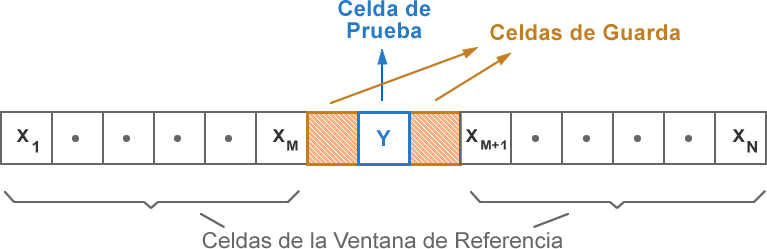
\includegraphics[scale=0.25]{./Figures/Estructura-del-Esquema-CA-CFAR.png}
\caption{Diagrama en bloques correspondiente al CA-CFAR.}
\label{fig:estructura_cfar}
\end{figure}

\subsection{Técnicas CA-CFAR relacionadas}

Para evitar introducir en la promediación la potencia proveniente de la celda bajo testeo, se establece alrededor de ella unas celdas de guarda, cuyo valor almacenado no se computa, sólo se transfiere a las celdas siguientes, como se ilustra en la figura \ref{fig:estructura_cfar}.

Existen variaciones inmediatas del algoritmo CA-CFAR \citep{CFAR_techniques}, en las cuales en lugar de considerar en la promediación de ruido los valores de ambas celdas de referencia, sólo se considera uno de ellos. Este es el caso de los algoritmos GOCA-CFAR (greatest of Cell-Averaging - CFAR) y SOCA-CFAR (smallest of Cell-Averaging - CFAR). Con estas técnicas se comparan los promedios parciales de las celdas de referencia y se considera el mayor o el menor respectivamente.

\subsection{Otras técnicas CFAR}
Existen otros algoritmos no considerados en este trabajo, que incorporan otras herramientas estadísticas, como ser OS-CFAR (por Ordered Statistic CFAR) y (TM-CFAR, por Trimmed Mean - CFAR):
\begin{itemize}
\item OS-CFAR
En la técnica CFAR de estadística ordenada, OS-CFAR, se ordenan las muestras de las celdas de referencia en orden ascendente. El elemento \(n/2\) es la mediana de los datos. El \(k-esimo\) elemento de la lista ordenada representa un determinado nivel de interferencia y el umbral es un múltiplo de este valor.
\item TM-CFAR
La técnica CFAR de constante media recortada (TM-CFAR), es una extensión de OS-CFAR en el que las celdas ordenadas en la ventana de referencia se recortan desde el extremo superior e inferior. El umbral es formado sumando las celdas restantes. En algunos TM-CFAR solo las celdas del extremo superior (celdas con mayor potencia) se descartan, por lo que si hay varios objetivos presentes en la ventana de referencia, el recorte elimina el efecto de la interferencia
objetivo.

\end{itemize}


\section{FPGA}

\begin{figure}
\centering
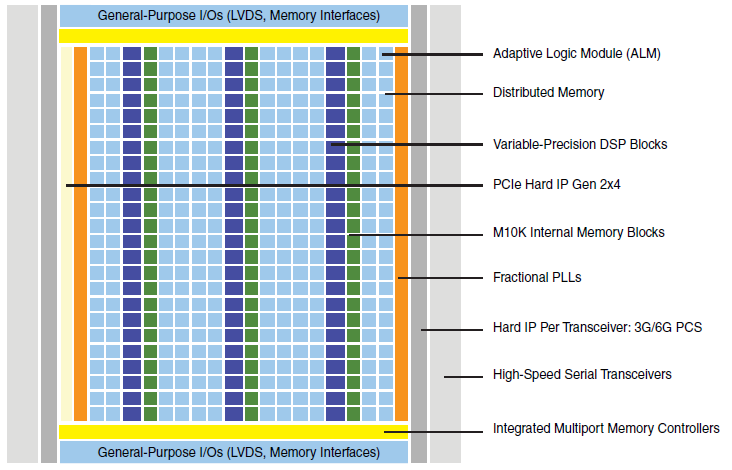
\includegraphics[scale=0.5]{./Figures/22-0.png}
\caption{Composición de una FPGA Cyclone V de Altera. Imagen tomada del Manual del chip.}
\label{fig:fpga_por_dentro}
\end{figure}

Las FPGA (por sus siglas en inglés, Field Programmable Gate Array) son una matriz de compuertas lógicas programables cuyos elementos se componen un conjunto de bloques lógicos configurables, conectados mediante conexiones programables \citep{FpgaArq}. Se crearon en el año 1984 como evolución de los dispositivos lógicos programables complejos (CPLD) y comparten ciertas similitudes con los Circuitos Integrados de Aplicación Específica, ASIC (acrónimo en inglés), sin embargo la diferencia con respecto a este viene marcada por su característica de ser reprogramable. También se pueden realizar comparaciones con otros dispositivos lógicos similares como GPP, DSP, ASIC estructurado, etc. Las FPGA se emplean en campos como la Medicina, procesamiento de imágenes y video, Aeroespacio y defensa, comunicaciones cableadas e inalámbricas, audio, entre otros \citep{fpga_xilinx}.

A diferencia con un microcontrolador, las FPGA no tiene una función específica incorporada, sino que poseen recursos para reproducir un circuito dentro del chip. Esto es posible debido los elementos lógicos individuales denominados CLBs (Configuble Logic Module) o  ALMs (Adaptative Logic Module), como se ilustra en la figura \ref{fig:fpga_por_dentro}. Las FPGA modernas incluyen en estos bloques elementos básicos como Flip Flops, Look-Up-Tables, Digital Signal Prossencing Blocks, relojes dedicados, PLLs, etc. Tambien tiene bloques de entrada y salida que se conectan con pines individuales de las ALMs, que pueden ejercer no sólo funciones de buffers sino también estados de alta impedancia.

Cabe mencionar que son dispositivos volátiles es decir que no tienen memoria, por sí solos no pueden almacenar su configuración de conexión y por tanto cuando se desconecta la fuente de energía se pierde esa configuración. Generalmente se utiliza una memoria por fuera de la FPGA para almacenar esa configuración.



\subsection{SoC-FPGA}

Los procesadores y las FPGA son dispositivos importantes en la mayoría de los sistemas embebidos. Los procesadores poseen la funcionalidad de gestión de alto nivel y las FPGA las estrictas operaciones en tiempo real, procesamiento de datos o funciones de interfaz.

Los dispositivos SoC-FPGA empezaron a producirse para brindar una alternativa de mayor desempeño y menor consumo y coste a sistemas que utilizan por separado una FPGA y un microprocesador o DSP. En los dispositivos SoC-FPGA se integra la arquitectura del procesador y FPGA en un sólo dispositivo. Esto brinda mayor integración, menor consumo de potencia, menor tamaño de placa y un mayor ancho de banda de comunicación entre el procesador y la FPGA \citep{soc_fpga}.

Como las señales entre el procesador y la FPGA ahora residen en el mismo chip, la comunicación entre los dos consume sustancialmente menos potencia en comparación con el uso de chips separados. Además la integración de miles de conexiones internas entre el procesador y la FPGA proporciona un ancho de banda mucho mayor y una latencia más baja que usar ambos dispositivos por separado.

El paso siguiente es incluir el chip dentro de una placa de circuito impreso (PCB, por el acrónimo inglés Printed Circuit Board). Para ellos hay empresas que ofrecen en el mercado PCB con diferentes tecnologías FPGA y variados periféricos. Un ejemplo es la placa tipo ADC-SoC, que incorpora una SoC-FPGA con un convertidor analógico a digital (ADC, por Analog to Digital Conveter) de alta velocidad.


\section{Bloques básicos de una FPGA}
En el presente trabajo se utilizó una FPGA de la firma Intel \citep{cycloneV_handbook}. A continuación se describe los componentes básicos que por generalmente incorpora una FPGA de esta empresa.

\subsection{ALM}

El bloque básico de una FPGA Cyclone V se denomina Adaptative Logic Module (ALM), el cual se ilustra en la figura \ref{ALM_diag_bloques}. Un ALM contiene cuatro registros programables, con los siguiente puertos:
\begin{itemize}
\item Data
\item Clock
\item Synchronous and asynchronous clear
\item Load
\end{itemize}

Las señales globales, los pines de entrada y salida de propósito general (GPIO)o cualquier señal interna de lógica pueden comandar las señales de control de clock y de clear de un registro ALM. Además los pines GPIO o la lógica interna controlan la señal de activación del reloj. Para las funciones combinacionales, los registros se omiten y la salida de la LUT es conducida directamente a las salidas de un ALM.

\begin{figure}
\centering
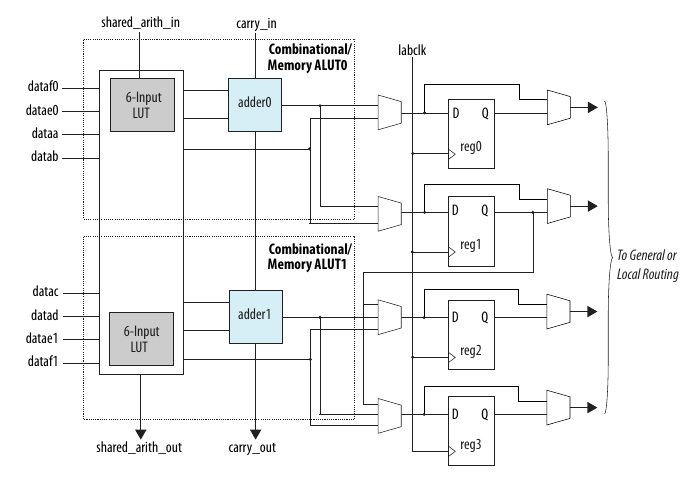
\includegraphics[scale=.75]{./Figures/diag_bloques_ALM.png}
\caption{Diagrama en bloques de un ALM. Imagen tomada del Manual del chip.}
\label{ALM_diag_bloques}
\end{figure}



\subsection{Bloques de memoria}

Posee además dos tipos de memorias embebidas, M10K y MLAB:

\begin{itemize}
\item
M10K: Las de tipo M10K son de 256 hasta 8000 bits de profundidad aproximadamente, están diseñadas para arrays extensos de memoria con puertos independientes.
\item
MLAB: Las de tipo MLAB sin embargo son de hasta 32 bits de profundidad y están optimizadas para la implementación de registros de desplazamientos, buffers tipo FIFO anchos y líneas de retardo. Cada MLAB se compone de diez ALMs y hasta el $25\%$ de las ALM se pueden configurar como memoria distribuida usando los bloques MLABs.
\end{itemize}

\subsection{Relojes y PLLs}
Posee 16 redes de reloj globales de 550 Mhz cuya arquitectura está basada en estructuras de Intel tipo globales, cuadrantes y periféricos. Esta estructura de reloj es compatible con pines de entrada de reloj dedicados y PLL fraccionales. Una característica importante del funcionamiento de los relojes es que en la herramienta Quartus identifica las secciones de la red de reloj sin usar y las desconecta, mejorando el consumo.


\subsection{Hard Processor System}
La FPGA posee integración con un sistema de procesamiento dentro del mismo chip. Este último se compone de una unidad de microprocesador con procesador córtex-A9 de ARM, controladores de memoria flash, soporte de periféricos y de interfaz, PLLs, interconexión SDRAM L3, entre otros.

Las partes HPS y FPGA del dispositivo SoC-FPGA son diferentes. El HPS arranca desde cualquiera de las múltiples fuentes de arranque, incluida la estructura FPGA y los dispositivos flash externos, y la FPGA se configura a través del HPS o cualquier fuente externa compatible con el dispositivo.





\section{Niveles de abstracción en el diseño digital}

En el ámbito del diseño digital se pueden distinguir diferentes niveles de abstracción \citep{niveles_abstraccion} que se distinguen por su impacto en el diseño y complejidad. Las decisiones a nivel conceptual son menos complejas pero tienen un impacto importante en el diseño final y a su vez la complejidad del diseño crece a medida que avanzamos en el ciclo del diseño. Podemos distinguir, por ejemplo, entre los siguientes niveles:

\begin{itemize}
\item
Nivel conceptual o de sistema:
Es el nivel más alto en el diseño. Consiste en captar los requerimientos y especificaciones del sistema y, a partir de los mismos, reducir opciones de diseño y algoritmos.

\item
Nivel algorítmico:
Consiste en implementar los algoritmos en lenguajes de alto nivel con la intención de determinar resultados sobre la viabilidad del diseño. Por ejemplo implementar una simulación usando lenguaje Python, lenguaje C/C++ o entorno MATLAB.
\item
Nivel de transferencia de registros:
En este nivel, también denominado RTL (por el acrónimo inglés, Register Transfer Level), se considera que el algoritmo ya está decidido y se procede a describir los detalles de cómo se mueven los datos entre y dentro de los subsistemas, además de cómo se manipulan los datos en función de las entradas del sistema. Su comportamiento se describe mediante un lenguaje de descripción de hardware (HDL, por el acrónimo de Hardware Description Language).
\item
Nivel de compuertas:
El código escrito en RTL se sintetiza para la implementación a nivel de compuerta. El proceso de síntesis toma el RTL y lo traduce, elaborando una lista de conexiones a nivel de puerta (netlist). Para la síntesis lógica, el usuario especifica restricciones de diseño y la tecnologı́a de destino en forma de una biblioteca de celdas estándar (cell library). La biblioteca tiene compuertas lógicas básicas estándar, como AND y OR, o macrocéldas como sumadores, multiplicadores, flip-flops, multiplexores, etc.
La herramienta convierte completamente el diseño descrito en RTL en un diseño que contiene celdas estándar. Para mapear de forma óptima la descripción de alto nivel en hardware real, la herramienta realiza varios pasos:
\begin{itemize}
\item
Convierte primero la descripción RTL en lógica booleana no optimizada.
\item
Realiza varias transformaciones para optimizar la lógica sujeto a restricciones de usuario, donde esta optimización es independiente de la tecnologı́a de destino.
\item
Finalmente, la herramienta mapea la lógica optimizada a celdas estándar específicas de la tecnología.
\end{itemize}


\item
Nivel de transistor
Es el nivel más bajo de abstracción, se describe el funcionamiento de las puertas y registros básicos utilizando transistores, cables y otros componentes eléctricos como resistencias y condensadores.

\end{itemize}



\section{Lenguaje de descripción de hardware}

Los lenguajes de descripción de hardware (HDL) se utilizan a nivel RTL para describir la estructura y comportamiento de sistemas digitales en forma textual. No son lenguajes de programación ya que a diferencia de estos, los HLDs pueden manejar múltiples procesos paralelos (como flip-flops y sumadores) que se ejecutan automáticamente de forma independiente entre sí. Cualquier cambio en la entrada del proceso activa automáticamente una actualización en la pila de procesos. En el proceso de diseño es importante tener en cuenta que cada línea de código representa uno o más componentes de hardware.
 
El uso de un lenguaje de descripción de hardware (HDL) para diseñar en dispositivos FPGA tiene las siguientes ventajas:
\begin{itemize}
\item
Enfoque de arriba hacia abajo (top-down) para proyectos grandes.
Este enfoque para el diseño de sistemas funciona bien para grandes proyectos que requieren que muchos diseñadores trabajen juntos. Una vez que el equipo de diseño determina el plan de diseño general, los diseñadores individuales pueden trabajar de forma independiente en secciones de código separadas.
\item
Simulación funcional al principio del flujo de diseño.
Probar la funcionalidad del diseño antes de que se implemente en el nivel RTL o en el nivel de puerta permite realizar los cambios necesarios desde el principio.

\item
Síntesis de código HDL para puertas. Sintetizando la descripción del hardware para apuntar a la implementación del dispositivo FPGA:

	\begin{itemize}
	\item
	Disminuye el tiempo de diseño al permitir una especificación de diseño de mayor nivel, en lugar de especificar el diseño a partir de los elementos base del dispositivo FPGA.
	\item
	Reduce los errores que pueden ocurrir durante una traducción manual de una descripción de hardware a un esquema de diseño.
	\item
	Permite que la herramienta de síntesis aplique técnicas de automatización (como los estilos de codificación y la inserción automática de entradas y salidas) durante la optimización del código original. Esto se traduce en una mayor optimización y eficiencia.
	\end{itemize}


\item
Permite probar diferentes implementaciones de diseño al principio del flujo de diseño. Utilizando la herramienta de síntesis para realizar la síntesis lógica y la optimización en puertas. Dado que el tiempo de síntesis es corto, se pueden explorar diferentes posibilidades arquitectónicas en el nivel de transferencia de registros (RTL).
\item
Reutilización del código de nivel de transferencia de registro (RTL).
Se puede reorientar el código de nivel de transferencia de registro (RTL) a nuevos dispositivos FPGA con mínimos cambios.
\item

\end{itemize}

Los lenguajes HDL soportados por la IEEE son Verilog-HDL y VHDL \citep{ieee_std} \citep{ieee_pkg}. VHDL es un lenguaje que inicialmente usaban los contratistas del Departamento de Defensa de EE.UU; ahora se usa comercialmente y en universidades de investigación. Verilog nació como un HDL exclusivo, promovido por una compañía llamada Cadence Data Systems, pero Cadence transfirió el control de Verilog a un consorcio de empresas y universidades llamado Open Verilog International (OVI). Actualmente OVI y Open VHDL Internacional se unieron para formar Accellera. Para este proyecto se empleó ambos lenguajes, los cuales se describirán a continuación.


\subsection{Aspectos básicos del lenguaje VHDL}
Un sistema digital está descrito por sus entradas y sus salidas y la relación que existe entre ellas \citep{intro_VHDL}. VHDL tiene una estructura que separa la declaración de puertos de entrada y de salida por un lado y por el otro la descripción del comportamiento del componente.
En la entidad (entity), se declaran los puertos de entrada y salida a utilizar, y en la sección arquitectura (architecture) se describe el comportamiento de la entidad, como se ilustra en la figura \ref{componente vhdl}. Cada arquitectura tiene asociada una entidad. Si es necesario, se pueden declarar bibliotecas a utilizar, por ejemplo para cálculo aritmético o para operación entre señales lógicas.

\subsubsection{Entidad de diseño}
La entidad de diseño es la principal abstracción en VHDL. Una entidad puede representar un sistema entero, un subsistema,una plaqueta, un chip, una macrocelda, una compuerta lógica o cualquier nivel de abstracción que se encuentre entre los antes mencionados.

Una entidad de diseño también puede describirse en términos de componentes interconectados. Cada componente de una entidad de diseño puede estar vinculada a una entidad de diseño de nivel inferior para definir la estructura o el comportamiento de ese componente, como se ilustra en la figura \ref{interconexión de componentes}. La separación de una entidad de diseño en componentes y la interconexión de esos componentes a otras entidades de diseño que pueden separarse de manera similar, da como resultado una jerarquía de entidades de diseño representando un diseño completo. Esta colección de entidades de diseño se denomina jerarquía de diseño. El bloque superior, denominado top-level, es un bloque externo y los bloques anidados en la jerarquía son bloques internos. El uso de jerarquías permite crear código reutilizable y crear componentes que realizan una función específica.

\begin{figure}
\centering
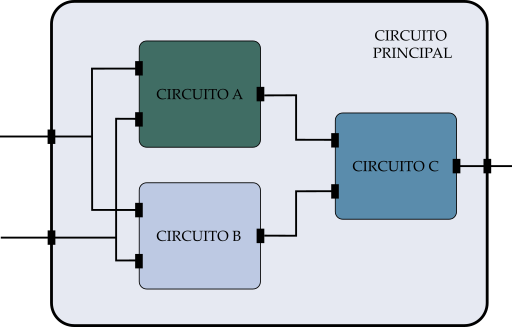
\includegraphics[scale=.5]{./Figures/vhdl_ejemplo2.png}
\caption{Circuitos A, B y C como instancias de un circuito principal.}
\label{interconexión de componentes}
\end{figure}


\subsubsection{Arquitectura de diseño}

La arquitectura define el cuerpo de una entidad de diseño. Especifica las relaciones entre las entradas y las salidas de esta, y puede estar expresada en términos de estructura, flujo de datos o comportamiento.


\begin{figure}
\centering
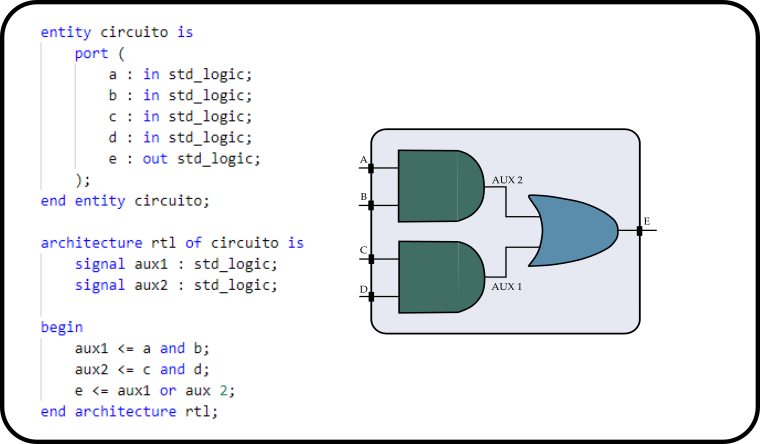
\includegraphics[scale=.65]{./Figures/vhdl_ejemplo.png}
\caption{Ejemplo de un componente descrito con VHDL.}
\label{componente vhdl}
\end{figure}

Dentro de la arquitectura se pueden crear las señales internas a esa entidad, que efectúan el proceso de las señales de entrada para proporcionar un cierto resultado en los puertos de salida. Para ello se utilizan procesos, asignaciones, instancias de componentes, registros y operaciones lógicas.

\begin{figure}
\centering
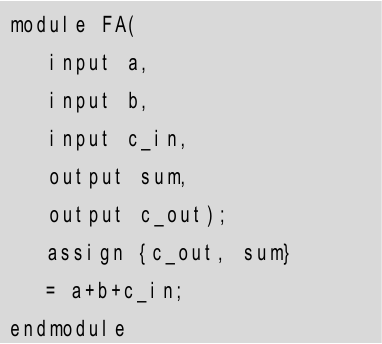
\includegraphics[scale=.95]{./Figures/verilog_ejemplo.png}
\caption{Ejemplo de un componente descrito con Verilog.}
\label{componente verilog}
\end{figure}

\subsection{Verilog}
Es un lenguaje de descripción de hardware que fue diseñado con una sintaxis similar a C. Puede operar a nivel RTL y de compuertas. El diseño se estructura mediante módulos,como se ilustra en la figura \ref{componente verilog}, que incluyen tanto declaración de puertos como el comportamiento.
Hay similitudes y diferencias en comparación con VHDL. Sin embargo, al parecer no hay una clara ventaja de usar uno u otro en términos de implementación.


\section{Flujo de diseno}
El diseño de un circuito digital involucra diferentes fases que se describen a continuación:

\subsection{Diseño}
Es la primer etapa del proceso. Consiste en ejecutar una toma de decisiones sobre el diseño a implementar y la manera de hacerlo. Esto implica tanto como determinar el tipo de placa, lenguaje HDL y herramientas a utilizar así como establecer jerarquías en el diseño y elaborar las especificaciones que deben cumplirse.


\subsection{Simulación}
Se utiliza una computadora para representar la estructura y comportamiento del sistema lógico digital \citep{morris_mano}. Mediante la simulación lógica, se interpreta la descripción HDL para predecir el comportamiento del hardware. De esta manera se pueden detectar errores en el funcionamiento del circuito antes de que se fabrique físicamente. Estos errores son corregidos modificando las sentencias del lenguaje empleado y sometiendo el diseño a un proceso de simulación. Una de las formas más usadas para simular diseños es el banco de pruebas (Testbench), que proporciona una forma gráfica de producir y visualizar las formas de onda de las señales de entrada y salida.



\begin{figure}
\centering

\includegraphics[scale=.5]{./Figures/test_bench3.png}
\caption{Diagrama en bloques de un test bench}
\label{diag test bench}
\end{figure}


El testbench no posee puertos de entrada ni de salida, sino señales de estimulación que se conectan a cada puerto de entrada del dispositivo bajo testeo o DUT (por el acrónimo inglés Device Under Test) y señales de observación que se conectar a los puertos de salida para observar la respuesta del DUT a esos estímulos, como se muestra en la figura \ref{diag test bench}.

Así, el proceso de simulación se resume en las siguientes etapas:

\begin{enumerate}
\item
Diseño del componente con HDL
\item
Diseño del marco de pruebas
\item
Verificación
\item
Corrección del componente
\end{enumerate}


\subsection{Síntesis}

En este proceso se emplea una herramienta de síntesis, proporcionada en general por el fabricante del chip, que elabora una lista de primitivas y sus interconexiones (netlist) a partir del diseño descrito en mediante HDL. La síntesis depende del dispositivo utilizado y de los recursos lógicos de los que disponga; diferentes dispositivos pueden implementar una misma función de distintas formas sin cambiar la funcionalidad del diseño. 

El grado de optimización del proceso de síntesis a la hora de convertir el código HDL al un circuito equivalente, depende de los siguientes factores:
\begin{enumerate}
\item La descripción del circuito.
Este punto es el más importante porque impacta en los recursos a utilizar y en las directivas a incluir. En la descripción además de decir qué función realiza el circuito, se describe la forma en la que debe realizarlo. Cuando se describe el funcionamiento de un circuito, existen muchas formas de hacer las mismas operaciones, y todas ellas darán lugar a distintas formas de implementación.

\item Los recursos disponibles en el dispositivo seleccionado.
Los recursos afectan a la forma en que las funciones descritas son interpretadas e implementadas en los bloques lógicos existentes en el dispositivo. Por ejemplo, un circuito que realice una división entre un número que no sea potencia de dos no podría hacerse en ciertos dispositivos, que no cuentan con esta característica.

\item Las directivas de síntesis seleccionadas por el diseñador.
Las directivas de síntesis son aquellos parámetros que se configuran para que la herramienta de síntesis los tenga en cuenta en el proceso de implementación. Por ejemplo, incluir restricciones de tiempo a ciertas señales permite que la implementación de los bloques que se conecten a dichas señales se realice de manera de ubicarlos en una sección del chip que permita que esta restricción se cumpla. En caso de que no se cumpla, la herramienta dará un error de síntesis para comunicar que el diseño debe ser modificado.
\end{enumerate}


\subsection{Implementación}
La implementación, también denominado como Place And Route (P \& R)en las FPGAs, consiste en situar el diseño sintetizado usando las celdas lógicas del dispositivo. La implementación transforma las Netlist de nivel medio creadas en la síntesis, y las mapea en la superficie de la FPGA, usando la lógica y los recursos internos disponibles. El archivo final es un Bitstream (.bit) que será el fichero final que se cargará en la FPGA.

\subsection{Configuración}
La configuración incluye la transferencia del fichero bitstream a la FPGA. Éste puede residir en una memoria no volátil como una PROM, o dentro de la FPGA (Muchas FPGA vienen con una memoria  interna capaz de mantener el fichero de configuración). El bitstream puede ser cargado en la FPGA mediante programación JTAG, a través de un procesador, microcontrolador u otro dispositivo externo.